\documentclass[12pt, a4paper]{article}

% --- PACKAGES ---
\usepackage[margin=1in]{geometry} % For setting page margins
\usepackage{amsmath}              % For advanced math environments
\usepackage[hidelinks]{hyperref}  % For clickable links
% Remove inputenc for modern TeX Live (UTF-8 is default)
\usepackage{booktabs}             % For professional-looking tables
\usepackage{times}                % Use Times New Roman font
\usepackage{newtxtext}            % Use newtxtext package
\usepackage{newtxtt}              % Provides matching typewriter font for Times
\usepackage{graphicx}             % For including graphics
\usepackage{pgfplots}
\pgfplotsset{compat=1.18}

% --- DOCUMENT METADATA ---
\title{A Performance-Based Analysis of ChatGPT on Competitive Programming Challenges: A Replication}
\author{Daniel Trimble}
\date{October 2, 2025}

% --- BEGIN DOCUMENT ---
\begin{document}

\maketitle

% --- ABSTRACT ---
\begin{abstract}
The integration of Large Language Models (LLMs) like ChatGPT into software development workflows has prompted significant discussion regarding their capabilities relative to human developers. While foundational studies have explored this relationship across a wide range of metrics, a need exists for focused, replicable performance benchmarks. This paper presents an agile replication of the work by Nascimento et al. (2023), concentrating specifically on the runtime and memory performance of ChatGPT-generated solutions on the LeetCode platform. I tested 30 problems of varying difficulty and compared the AI's "out-of-the-box" solutions against the platform's median developer benchmarks. The results indicate that ChatGPT \textbf{consistently} generates code that executes faster than most human submissions in terms of runtime performance, with a median percentile of 87.04\%, but demonstrates only average memory efficiency (median memory percentile: 54.32\%). A clear trend emerges where runtime performance, while still strong, degrades significantly \textbf{as problem complexity increases}---that is, as the LeetCode problem difficulty shifts from Easy to Medium to Hard (see Appendix~\ref{sec:example_problems} for representative examples). These findings contribute to a more nuanced understanding of the practical strengths and weaknesses of current-generation AI in performance-critical programming tasks.
\end{abstract}

% --- SECTIONS ---
\section{Introduction}

The proliferation of advanced AI, particularly LLMs, is rapidly changing the landscape of software engineering. Tools like ChatGPT are now widely used for code generation, debugging, and ideation. However, empirical validation of their performance against skilled human developers is still an emerging area of research. This study seeks to contribute to this area by providing a focused performance analysis.

Building on the comprehensive, multi-faceted methodology of Nascimento et al. (2023), this paper narrows its scope to answer three specific questions:
\begin{enumerate}
    \item \textbf{Runtime Performance:} Does ChatGPT's generated code execute faster than 50\% of human submissions on LeetCode?
    \item \textbf{Memory Efficiency:} Is its code more memory-efficient than 50\% of submissions?
    \item \textbf{Consistency:} How does its performance vary across Easy, Medium, and Hard problems?
\end{enumerate}
By concentrating on these objective, platform-provided metrics, I aim to deliver a clear and replicable benchmark of ChatGPT's capabilities.

\section{Background: The Original Study}

My research is a direct response to the foundational work "Comparing Software Developers with ChatGPT: An Empirical Investigation" (Nascimento et al., 2023). In their study, the authors conducted a broad comparison of ChatGPT-generated code against human solutions. Their methodology was notable for its holistic approach, analyzing not only performance (runtime) but also crucial non-functional requirements such as code quality, security vulnerabilities, and energy efficiency.

The key conclusion from their work was that while AI is a powerful tool for code generation, it cannot be seen as a direct replacement for human developers. They found that AI-generated solutions often failed on the critical non-functional requirements where human experience and oversight are essential. Their study advocated for a collaborative model of human-AI interaction in software development.

\section{Methodology}

To investigate my research questions, I adopted a quantitative, comparative methodology consisting of three stages.

\subsection{Problem Selection}
A set of 30 problems was curated from the LeetCode platform. The selection was stratified to ensure a balanced sample: 10 "Easy," 10 "Medium," and 10 "Hard" problems. The set was further diversified to cover a range of common computer science topics.

\subsection{Data Collection}
For each of the 30 problems, a solution was generated using ChatGPT version 4.1, accessed via an embedded agent within the Visual Studio Code editor. A standardized, non-optimized prompt was used for each problem to request a solution in JavaScript. The first complete solution provided by the model was submitted to the LeetCode online judge without any human modification. The resulting runtime (\texttt{time\_pct}) and memory usage (\texttt{space\_pct}) percentile rankings were recorded. The full step-by-step workflow for this process is illustrated in Appendix~\ref{sec:submission_flow}.

\subsection{Analysis Protocol}
The collected percentile rankings serve as my primary data. A ranking of 80\% means the solution was faster or more memory-efficient than 80\% of all other successful submissions.

\textbf{Benchmark:} LeetCode provides percentile rankings for both runtime and memory usage by comparing each submission to all other successful submissions for the same problem. Since the vast majority of these are from human users, the percentile metric inherently benchmarks AI-generated solutions against a large, diverse pool of human developers. Thus, a percentile of 80\% means the solution is faster (or more memory-efficient) than 80\% of all human submissions for that problem. This built-in comparison forms the baseline for this experiment, eliminating the need for a separate human control group.

\section{Results}

A significant preliminary finding, before analyzing performance percentiles, was the reliability and speed of the solution generation. For all 30 problems, regardless of difficulty, the first solution generated by ChatGPT was accepted by the LeetCode judge on the first submission. This 100\% first-try acceptance rate demonstrates a high degree of functional correctness for the given problems.

The data revealed a clear distinction between ChatGPT's runtime performance and its memory efficiency.

\subsection{Aggregate Runtime Performance}
The AI-generated solutions were exceptionally fast. The aggregate runtime performance across all 30 problems was significantly higher than the median developer.
\begin{itemize}
    \item The mean runtime percentile was 76.74\%.
    \item The median runtime percentile was 87.04\%.
\end{itemize}

\subsection{Aggregate Memory Performance}
In contrast, the aggregate memory efficiency of the solutions was average, hovering just above the 50th percentile baseline.
\begin{itemize}
    \item The mean memory percentile was 54.36\%.
    \item The median memory percentile was 54.32\%.
\end{itemize}

\subsection{Performance by Problem Difficulty}
Disaggregating the results by problem difficulty uncovered a strong, inverse correlation between problem complexity and runtime performance. While still performing above average, the AI's speed advantage diminished as problems became harder. This is likely because harder LeetCode problems require more complex, multi-step reasoning or the application of advanced algorithms, which may exceed the model's ability to generate optimal solutions without iterative refinement or additional guidance. Memory performance did not show a similar clear trend.

Figure~\ref{fig:scatter_difficulty_chart} provides a visualization of the raw runtime and memory percentiles for each problem, grouped by difficulty. This scatter plot highlights the spread and clustering of performance across the dataset.

\begin{table}[h!]
\centering
\caption{Performance Percentiles by Difficulty}
\label{tab:difficulty_performance}
\begin{tabular}{@{}lcccc@{}}
\toprule
\textbf{Difficulty} & \textbf{Avg. Runtime} & \textbf{Median Runtime} & \textbf{Avg. Memory} & \textbf{Median Memory} \\ \midrule
Easy (n=10)   & 95.34\% & 100.00\% & 48.49\% & 54.32\% \\
Medium (n=10) & 68.80\% & 78.42\% & 57.81\% & 56.13\% \\
Hard (n=10)   & 61.93\% & 58.42\% & 54.76\% & 52.51\% \\ \bottomrule
\end{tabular}
\end{table}

\begin{figure}[h!]
\centering
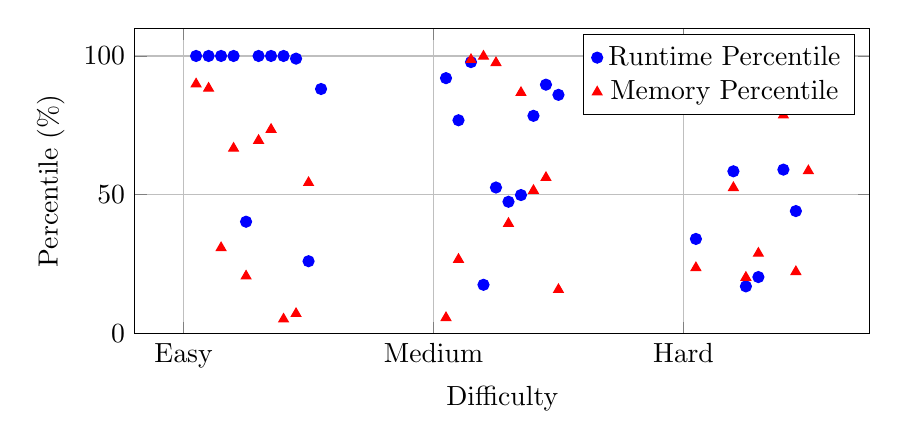
\begin{tikzpicture}
\begin{axis}[
    width=0.9\textwidth,
    height=0.45\textwidth,
    xlabel={Difficulty},
    ylabel={Percentile (\%)},
    xtick={1,2,3},
    xticklabels={Easy, Medium, Hard},
    ymin=0, ymax=110,
    legend style={at={(0.98,0.98)},anchor=north east},
    grid=major
]
% Runtime Percentile (blue dots, jittered)
\addplot[
    color=blue,
    only marks,
    mark=*,
] coordinates {
    (1.05,100) (1.10,100) (1.15,100) (1.20,100) (1.25,40.24) (1.30,100) (1.35,100) (1.40,100) (1.45,99.04) (1.50,26) (1.55,88.09)
    (2.05,92) (2.10,76.82) (2.15,97.79) (2.20,17.5) (2.25,52.57) (2.30,47.43) (2.35,49.85) (2.40,78.42) (2.45,89.65) (2.50,85.98)
    (3.05,34.03) (3.10,100) (3.15,97.63) (3.20,58.42) (3.25,16.93) (3.30,20.29) (3.35,100) (3.40,59.02) (3.45,44.08) (3.50,88.91)
};
\addlegendentry{Runtime Percentile}

% Memory Percentile (red triangles, jittered)
\addplot[
    color=red,
    only marks,
    mark=triangle*,
] coordinates {
    (1.05,89.89) (1.10,88.34) (1.15,30.84) (1.20,66.7) (1.25,20.62) (1.30,69.53) (1.35,73.51) (1.40,5.11) (1.45,7.09) (1.50,54.32)
    (2.05,5.62) (2.10,26.64) (2.15,98.66) (2.20,99.89) (2.25,97.55) (2.30,39.6) (2.35,86.79) (2.40,51.48) (2.45,56.13) (2.50,15.76)
    (3.05,23.64) (3.10,89.17) (3.15,89.3) (3.20,52.51) (3.25,20.15) (3.30,28.84) (3.35,84.5) (3.40,78.65) (3.45,22.22) (3.50,58.59)
};
\addlegendentry{Memory Percentile}

\end{axis}
\end{tikzpicture}
\caption{Scatter plot of raw runtime and memory percentiles by difficulty (jittered for visibility)}
\label{fig:scatter_difficulty_chart}
\end{figure}

\section{Discussion}

\subsection{Interpretation of Findings}
The results of this study are twofold. First, and most clearly, ChatGPT excels at generating code that is highly optimized for execution speed. A median runtime percentile of 87.04\% suggests that its "out-of-the-box" solutions are faster than the vast majority of human submissions on LeetCode. This is likely because the model has been trained on a massive corpus of optimized code, allowing it to recognize and implement efficient algorithms for common problems.

Second, this speed advantage is not absolute and is highly dependent on task complexity. The dramatic drop in average runtime performance from 95.34\% on "Easy" problems to 61.93\% on "Hard" problems is the most significant finding of this paper. It indicates that while ChatGPT can produce near-perfect solutions for standard, well-defined problems---that is, problems sourced from LeetCode, a widely used platform for competitive programming with clearly specified inputs and outputs---its ability to optimize for novel or multi-step algorithmic challenges is less reliable.

In contrast, its memory performance is consistently average. This suggests that the model does not prioritize memory optimization to the same degree as runtime, often settling for standard data structures that are functionally correct but not necessarily the most memory-efficient.

It is critical to contextualize the finding of average memory performance. Unlike a fixed algorithm, an LLM's output is malleable. A developer could trivially follow up with a prompt such as, "Refactor this code to be more memory-efficient," and likely receive a superior solution. This underscores a key insight into the evolving role of developers: the key to leveraging LLMs effectively will not just be in generating initial code, but in managing expectations and iteratively refining the output. Future developers will benefit from strong prompt engineering skills and, critically, from implementing robust test automation for load and performance.

\subsection{Limitations}
This study has three primary limitations. First, its scope is restricted to performance and does not analyze code quality, security, or maintainability. Second, I only tested the first, unoptimized solution from the AI. Third, the LeetCode ranking system is a "black box," and the exact dataset for comparison is unknown.

\section{Conclusion and Future Work}

This study provided a focused performance benchmark of ChatGPT on competitive programming tasks. My results indicate that \textbf{ChatGPT is a remarkably capable tool for generating highly efficient code in terms of speed on the first pass, though its solutions typically consume an average amount of memory compared to human submissions.} The model's primary weakness appears to be a degradation in runtime optimization as problem complexity increases.

This confirms the core thesis of Nascimento et al. (2023): AI is a powerful collaborator, not a replacement for human developers. A human developer's role may shift towards guiding the AI, verifying its output, and performing the complex, nuanced optimization on difficult problems where the AI is less effective.

Future work should expand upon this analysis to include the non-functional requirements. Comparing different LLMs and analyzing the impact of prompt engineering on performance would also be valuable next steps.

\section{References}

Nascimento, N., Alencar, P., \& Cowan, D. (2023). \textit{Comparing Software Developers with ChatGPT: An Empirical Investigation}. arXiv preprint arXiv:2305.11837. \url{https://arxiv.org/pdf/2305.11837}

\appendix
\section{Example Problems and Solutions}
\label{sec:example_problems}

This appendix provides representative examples of LeetCode problems used in this study, including their official difficulty level and the corresponding solution generated by ChatGPT (version 4.1, JavaScript). Each example includes the problem title, difficulty, and the unmodified code submitted to LeetCode.

\subsection{Example 1: Two Sum}
\textbf{LeetCode ID: 1} \\
\textbf{Title: Two Sum} \\
\textbf{Difficulty: Easy}

\textbf{Problem Description:}
Given an array of integers \texttt{nums} and an integer \texttt{target}, return indices of the two numbers such that they add up to \texttt{target}.

\textbf{ChatGPT Solution (JavaScript):}

\begin{verbatim}
function twoSum(nums, target) {
    const map = new Map();
    for (let i = 0; i < nums.length; i++) {
        const complement = target - nums[i];
        if (map.has(complement)) {
            return [map.get(complement), i];
        }
        map.set(nums[i], i);
    }
}
\end{verbatim}

\subsection{Example 2: Add Two Numbers}
\textbf{LeetCode ID: 2} \\
\textbf{Title: Add Two Numbers} \\
\textbf{Difficulty: Medium}

\textbf{Problem Description:}
You are given two non-empty linked lists representing two non-negative integers. The digits are stored in reverse order, and each of their nodes contains a single digit. Add the two numbers and return the sum as a linked list.

\textbf{ChatGPT Solution (JavaScript):}

\begin{verbatim}
function addTwoNumbers(l1, l2) {
    let dummy = new ListNode(0);
    let curr = dummy;
    let carry = 0;
    while (l1 || l2 || carry) {
        let sum = (l1 ? l1.val : 0) + (l2 ? l2.val : 0) + carry;
        carry = Math.floor(sum / 10);
        curr.next = new ListNode(sum % 10);
        curr = curr.next;
        if (l1) l1 = l1.next;
        if (l2) l2 = l2.next;
    }
    return dummy.next;
}
\end{verbatim}

\subsection{Example 3: Median of Two Sorted Arrays}
\textbf{LeetCode ID: 4} \\
\textbf{Title: Median of Two Sorted Arrays} \\
\textbf{Difficulty: Hard}

\textbf{Problem Description:}
Given two sorted arrays \texttt{nums1} and \texttt{nums2} of size \texttt{m} and \texttt{n} respectively, return the median of the two sorted arrays. The overall run time complexity should be $O(\log(m+n))$.

\textbf{ChatGPT Solution (JavaScript):}

\begin{verbatim}
function findMedianSortedArrays(nums1, nums2) {
    if (nums1.length > nums2.length) {
        return findMedianSortedArrays(nums2, nums1);
    }
    const m = nums1.length;
    const n = nums2.length;
    let imin = 0, imax = m, halfLen = Math.floor((m + n + 1) / 2);
    while (imin <= imax) {
        let i = Math.floor((imin + imax) / 2);
        let j = halfLen - i;
        if (i < m && nums2[j - 1] > nums1[i]) {
            imin = i + 1;
        } else if (i > 0 && nums1[i - 1] > nums2[j]) {
            imax = i - 1;
        } else {
            let maxOfLeft;
            if (i === 0) {
                maxOfLeft = nums2[j - 1];
            } else if (j === 0) {
                maxOfLeft = nums1[i - 1];
            } else {
                maxOfLeft = Math.max(nums1[i - 1], nums2[j - 1]);
            }
            if ((m + n) % 2 === 1) {
                return maxOfLeft;
            }
            let minOfRight;
            if (i === m) {
                minOfRight = nums2[j];
            } else if (j === n) {
                minOfRight = nums1[i];
            } else {
                minOfRight = Math.min(nums1[i], nums2[j]);
            }
            return (maxOfLeft + minOfRight) / 2.0;
        }
    }
    throw new Error("Input arrays are not sorted or invalid");
}
\end{verbatim}

\section{Appendix: Solution Generation and Submission Flow}
\label{sec:submission_flow}

This appendix visually documents the end-to-end process used to generate and submit solutions in this study. The flow proceeds as follows:

\begin{enumerate}
    \item \textbf{Problem Selection on LeetCode:} The user browses and selects a problem to solve.\\
    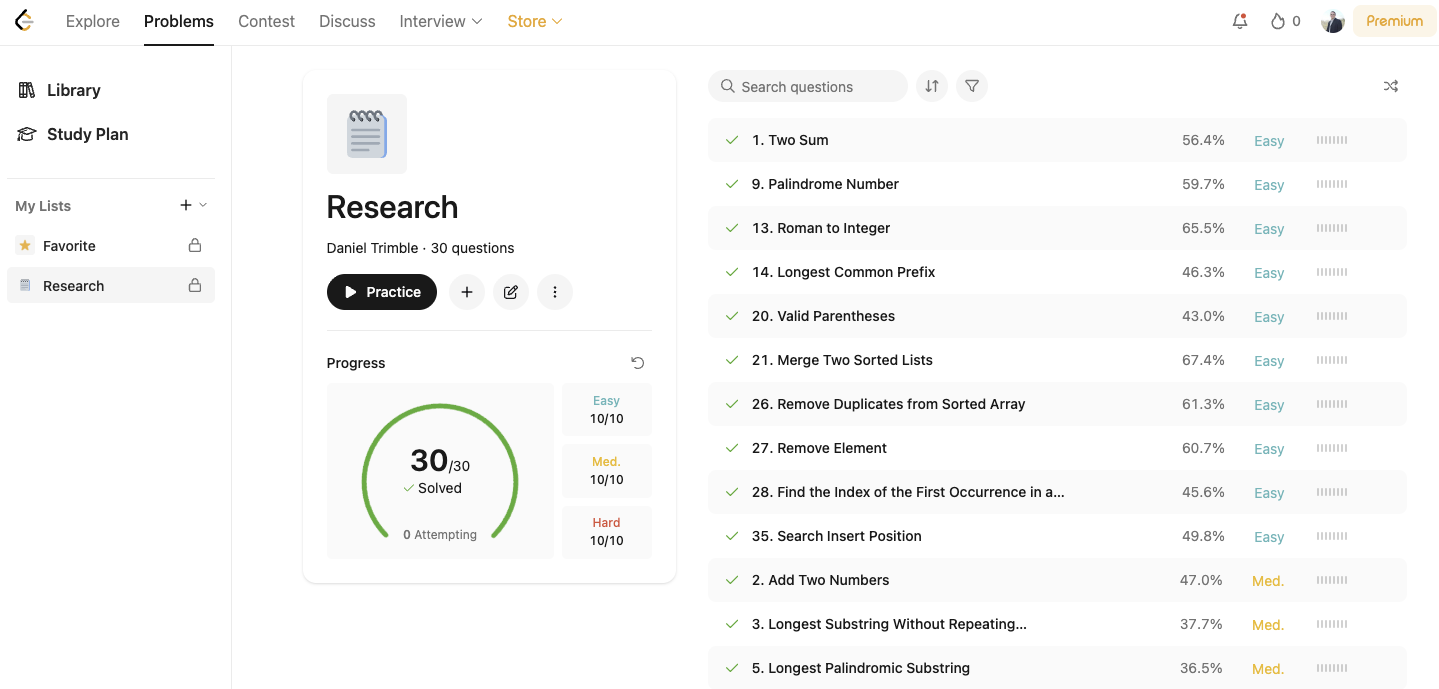
\includegraphics[width=0.9\textwidth]{leetcode1.png}
    \item \textbf{Viewing the Problem Details:} The full problem description and constraints are reviewed.\\
    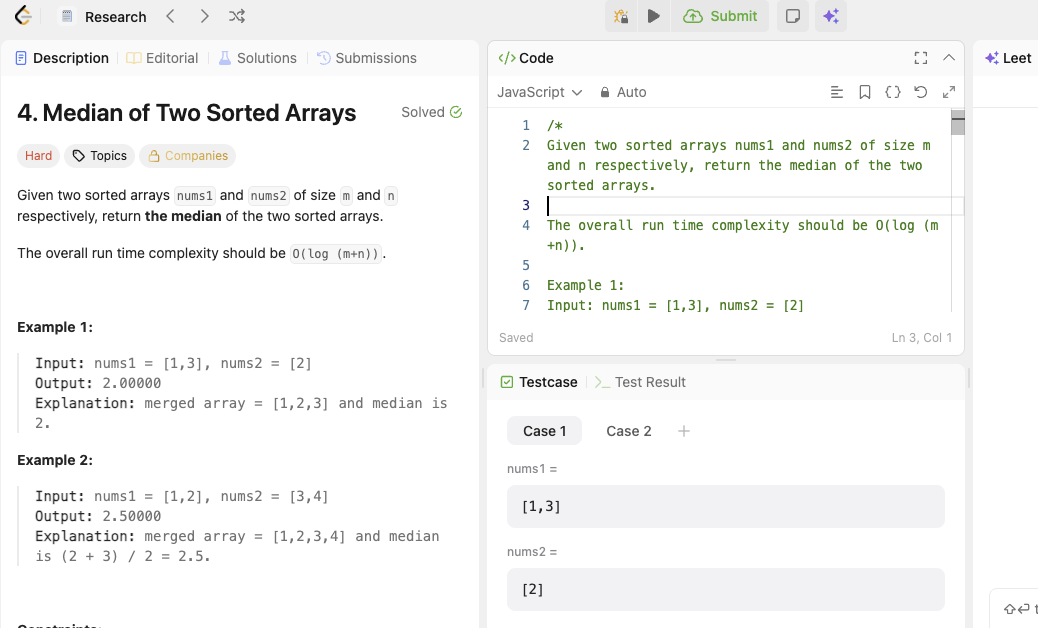
\includegraphics[width=0.9\textwidth]{leetcode2.png}
    \item \textbf{Solution Generation in VS Code (Step 1):} The user prompts ChatGPT within Visual Studio Code to generate a solution.\\
    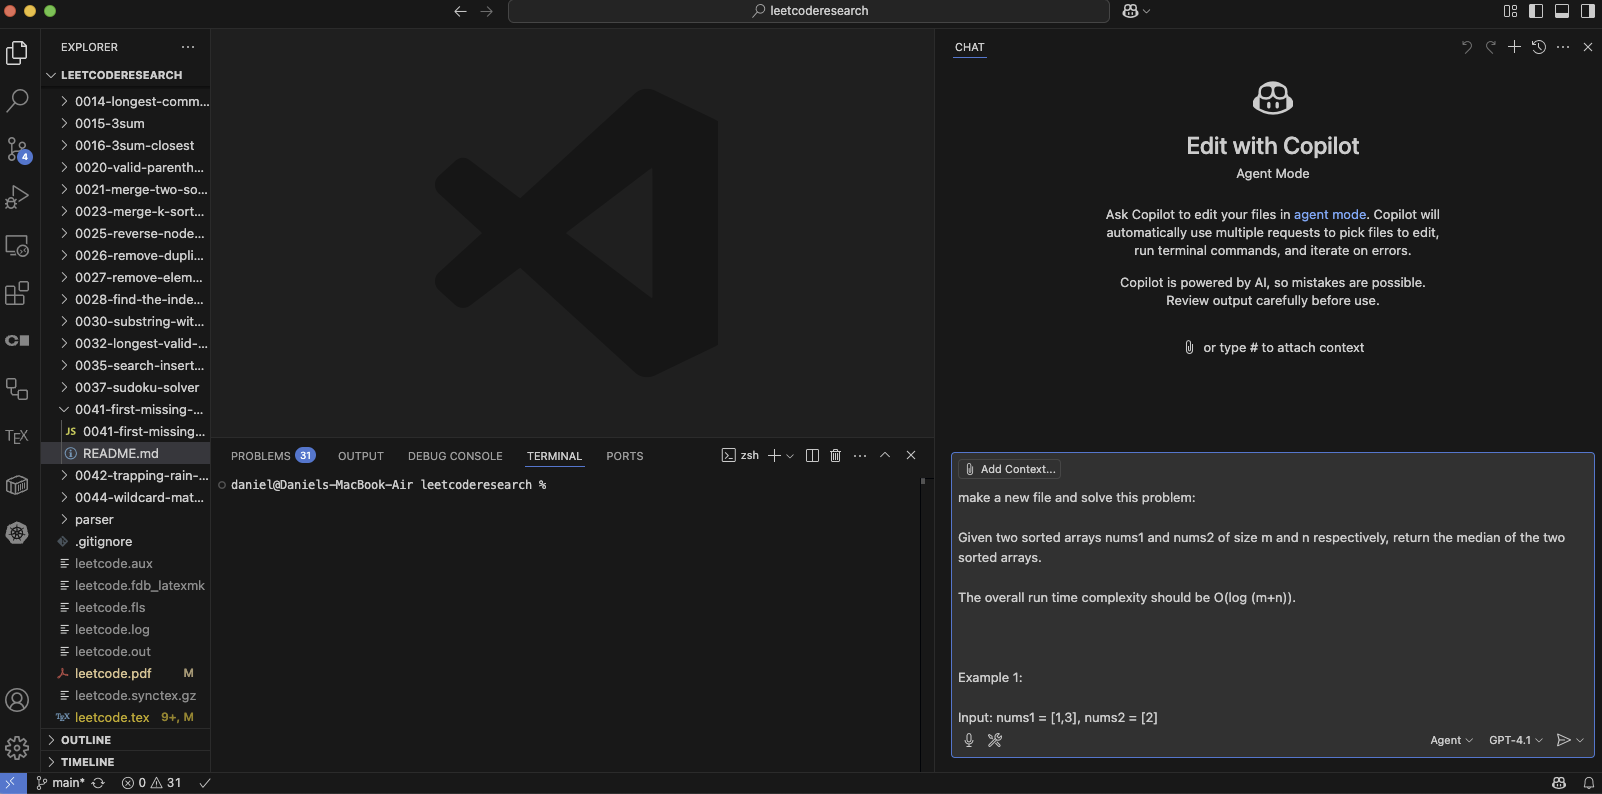
\includegraphics[width=0.9\textwidth]{vscode1.png}
    \item \textbf{Solution Generation in VS Code (Step 2):} The generated code is reviewed and prepared for submission.\\
    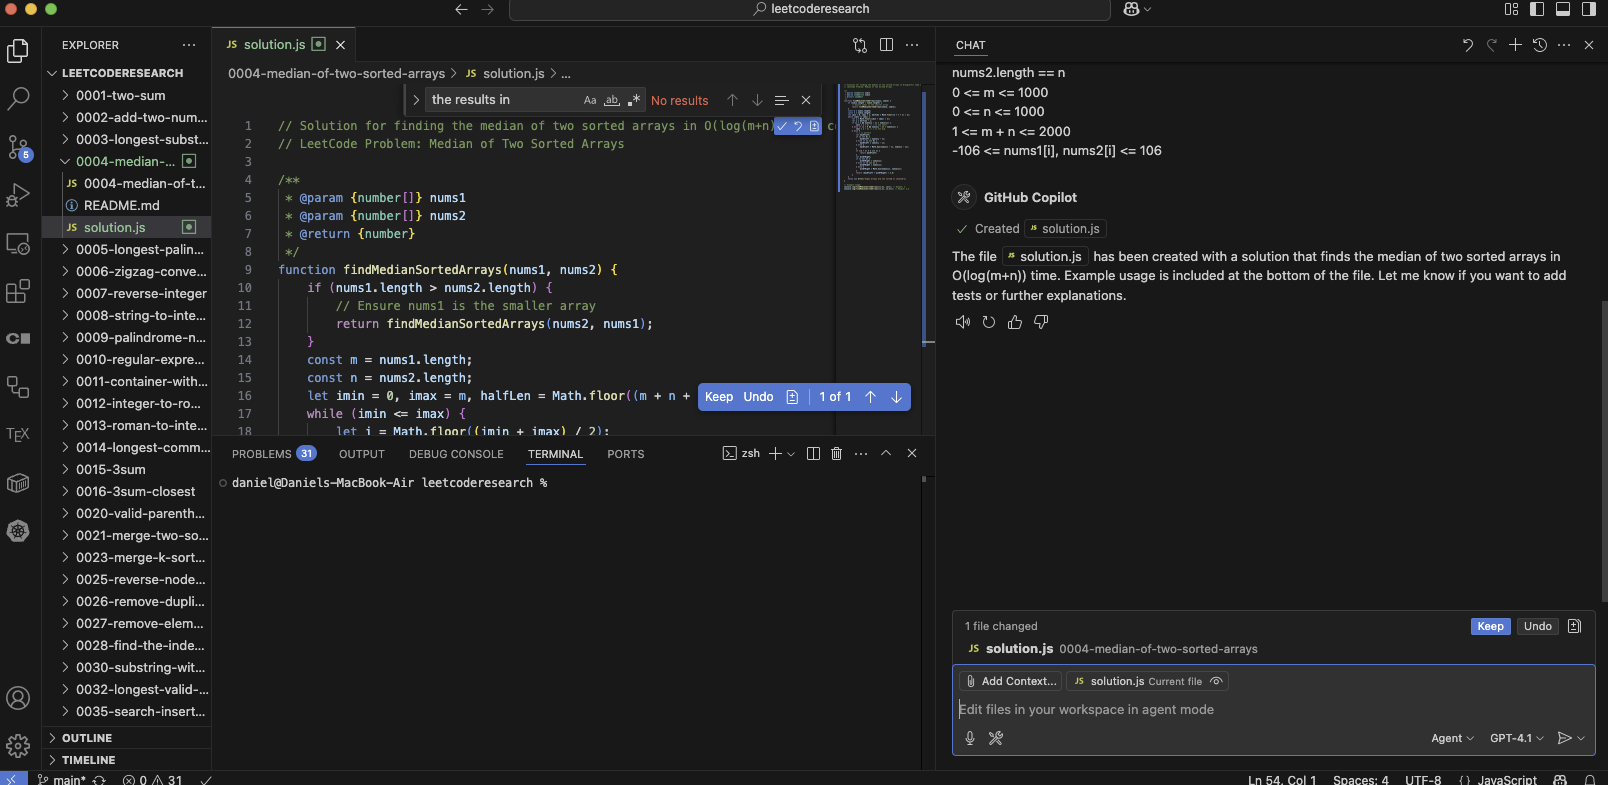
\includegraphics[width=0.9\textwidth]{vscode2.png}
    \item \textbf{Submission and Acceptance:} The solution is submitted to LeetCode and accepted by the online judge.\\
    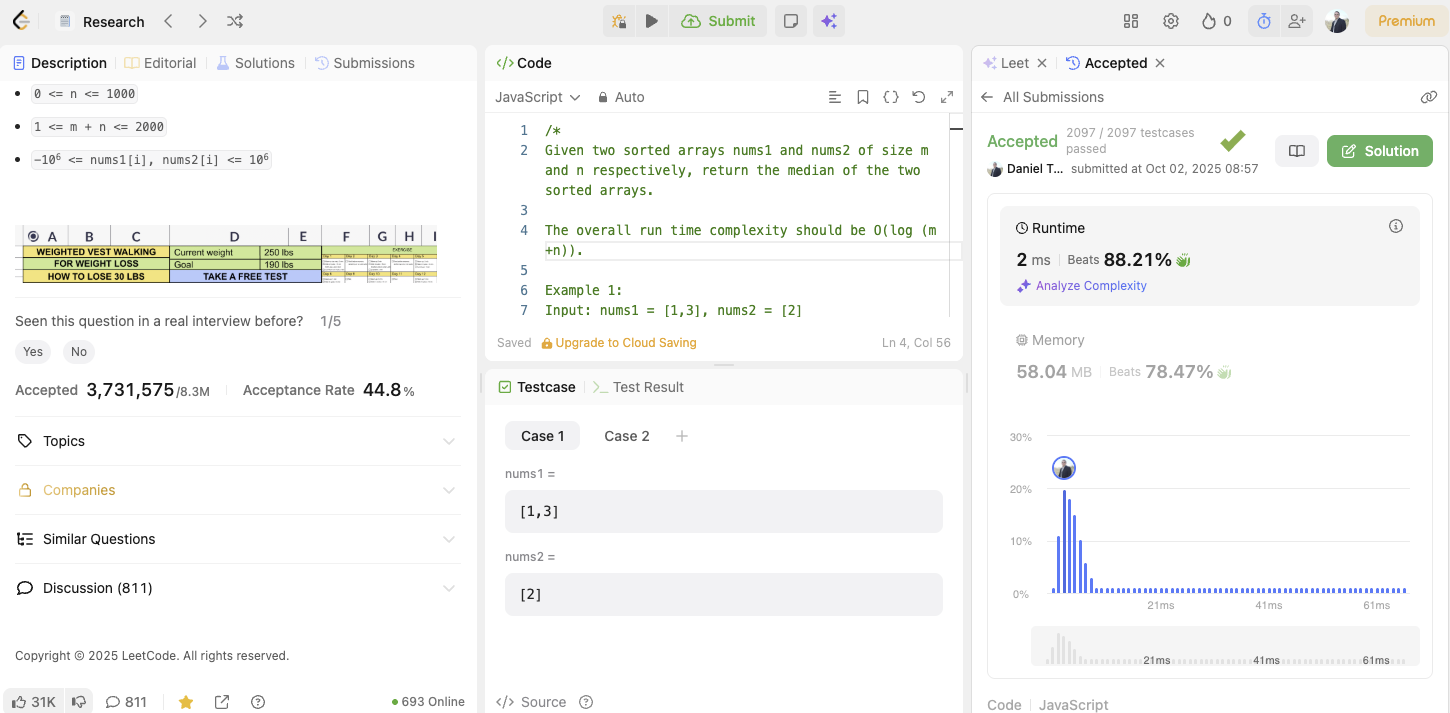
\includegraphics[width=0.9\textwidth]{leetcodesubmitted.png}
\end{enumerate}

This workflow ensures a consistent, replicable process for evaluating AI-generated solutions against the LeetCode benchmark.

\end{document}

